\documentclass{article}

%\usepackage[draft]{todonotes}
\usepackage{xcolor}
\usepackage[utf8]{inputenc}
\usepackage{mathtools}
\usepackage[utf8]{inputenc}
\usepackage[T1]{fontenc}
\usepackage[english]{babel}
\usepackage{graphicx}
%\usepackage{caption}
\usepackage{subcaption}
\usepackage{fixltx2e}
\usepackage{float}
\usepackage{amsthm}
\usepackage{amssymb}
\usepackage{booktabs}
\usepackage{enumitem} 
\newtheorem{definition}{Definition}
\newtheorem{theorem}{Theorem}
\usepackage{placeins}
\usepackage[a4paper, total={6in, 10in}]{geometry}


\numberwithin{equation}{subsection}
\setlength\parindent{0pt}
\setcounter{tocdepth}{2}

\begin{document}
	
	\section{Logistic-Linear Growth}
	
	Figure \ref{fig::NMutstime1} shows the evolution of the population size and the inferred mutation rate over time for $ \mu = 2$. Both these values are normed for comparability: The population size is divided by $N$, while the inferred mutation rate is divided by the true mutation rate and by a factor of 2 (to account for the simulations being only symmetric reproduction events). I then fitted the lines from time point 20-50, because that's when the inferred mutation rate seems to enter a linear phase. It can be seen that while there is an early fast-growing phase, the linear fit is very good for both values, and the slopes look quite close.For other values of $\mu$, this plot looks pretty much exactly identical, except for very slight variance.\\
	\\
	Figure \ref{fig::NMutsInf} shows the slope of the fitted lines from figure \ref{fig::NMutstime1} for different values of $\mu$, ranging from $0.2$ to $2$. As suspected, the population growth and the slope of the inferred mutation rate are quite close, though the latter is very slightly but consistently higher. The true $\mu$ however seems to have absolutely no influence on the relative slope.\\
	\\
	Lastly, we can see a few VAF-distributions for different time points in figure \ref{fig::VAFtimeline}. At $ t = 1$ and $2$, the distribution looks quite close to $ 1/f^2$. From $ t \geq 10 $, it's already very close to $1/f$. Only around $ t=5$, it seems to be in the middle.
	


	\begin{figure}[h!]
	\centering
	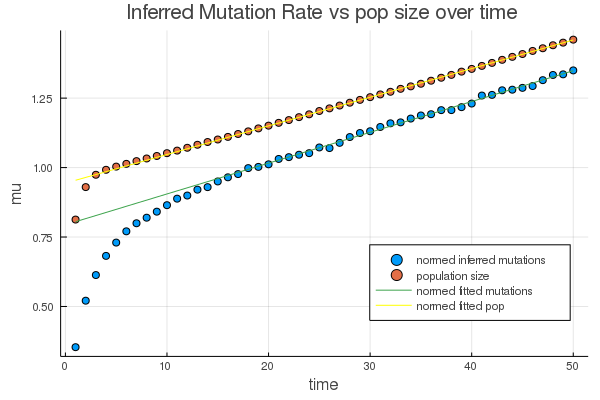
\includegraphics[width=\linewidth]{LogLinInfMutRate_N200_t50_mu2.png}
	
	\caption{On the y-Axis, normed population size $N(t)/N_{max}$ in red compared to the normed inferred mutation rate $ inf_\mu(t)/\mu_{true}/2$ in blue. On the x-Axis, time. Parameters: $ N_{max} = 200$, $\mu = 2 $, $ S = 100 $.}
	\label{fig::NMutstime1}
	\end{figure}
	
	
	
	\begin{figure}[h!]
		\centering
		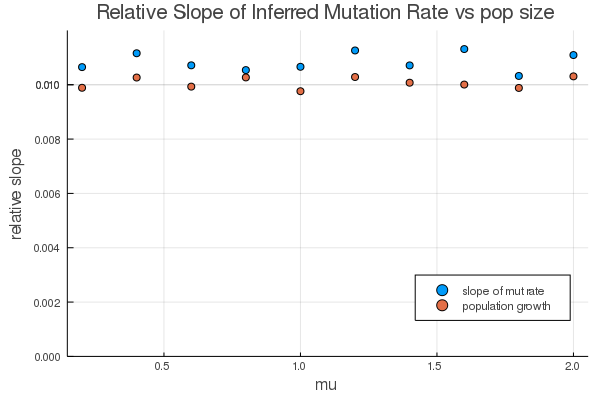
\includegraphics[width=\linewidth]{LogLinInfMutRate_N200_t50.png}
		
		\caption{On the y-Axis, slope of the increase of either the normed population size $N(t)/N_{max}$ in red compared to the normed inferred mutation rate $ inf_\mu(t)/\mu_{true}/2$ in blue. On the x-Axis, the true mutation rate. Parameters: $ N_{max} = 200$, $\mu = 2 $, $ S = 100 $.}
		\label{fig::NMutsInf}
	\end{figure}

	\begin{figure}[h!]
	\centering
	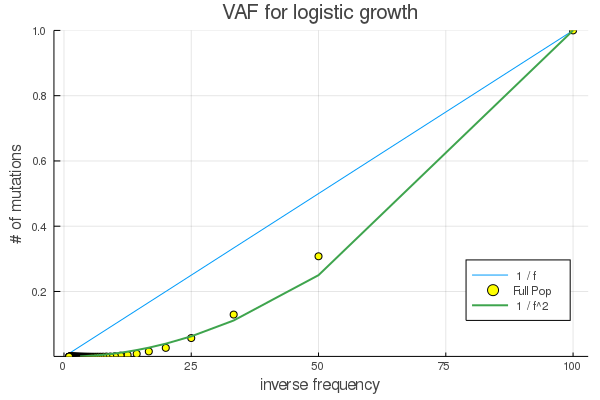
\includegraphics[width=0.32\linewidth]{VAFtimeline/LogLinVAF_N200_mu2_t1.png}
	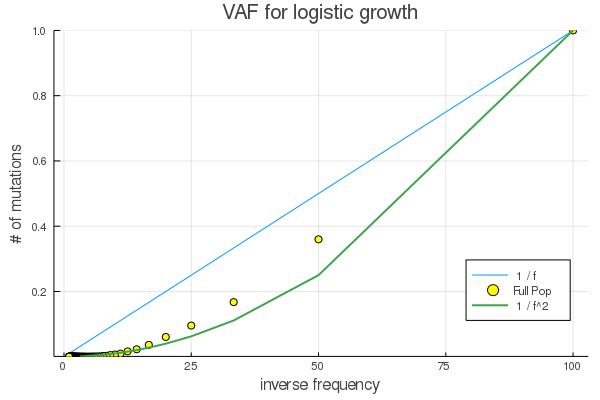
\includegraphics[width=0.32\linewidth]{VAFtimeline/LogLinVAF_N200_mu2_t2.png}
	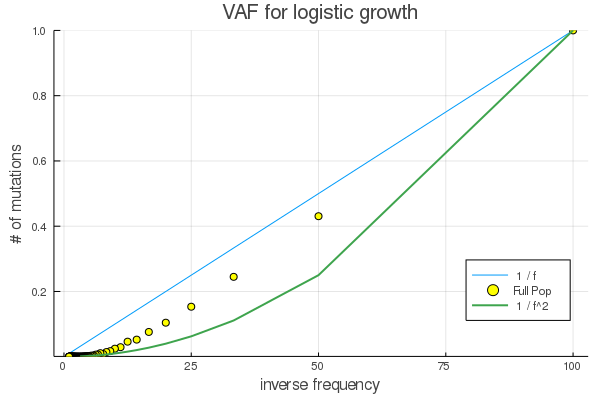
\includegraphics[width=0.32\linewidth]{VAFtimeline/LogLinVAF_N200_mu2_t5.png}
	
	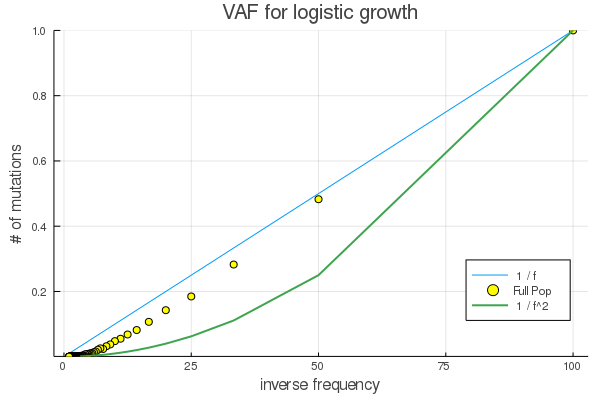
\includegraphics[width=0.32\linewidth]{VAFtimeline/LogLinVAF_N200_mu2_t10.png}
	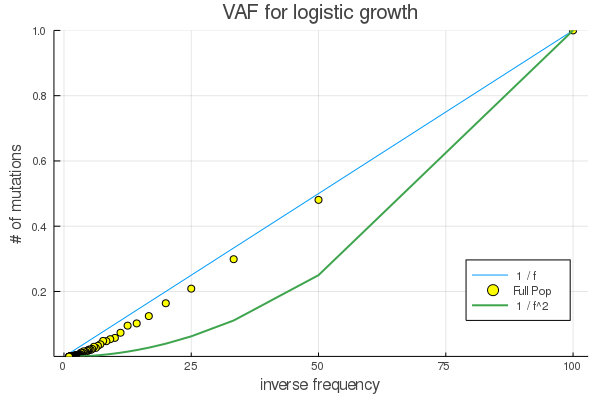
\includegraphics[width=0.32\linewidth]{VAFtimeline/LogLinVAF_N200_mu2_t20.png}
	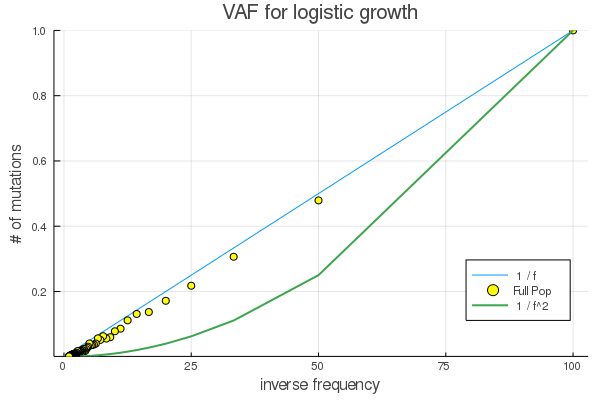
\includegraphics[width=0.32\linewidth]{VAFtimeline/LogLinVAF_N200_mu2_t50.png}
	
	\caption{These figures show the VAF-distribution for various time points, increasing from upper left to lower right. Parameters: $ N_{max} = 200$, $\mu = 2 $, $ S = 100 $, $ t = \{1,2,5,10,20,50\}$.}
	\label{fig::VAFtimeline}
	\end{figure}

\end{document}